\newpage
\chapter{Fokusace - teorie} 
\label{kapFok}

Fokusace a urychlování svazku byly realizovány pomoci elektronové optiky, soustavy elektrostatických čoček - několika cylindrických elektrod na které se přivádí různé napětí.  

Princip funkce elektrostatických čoček se dá ukázat na příkladě tzv. einzelových čoček - neurychlující fokusující soustavy třech cylindrických elektrod, ve které boční elektrody jsou pouze uzemněné a na elektrodu uprostřed je přivedeno napětí (Obr. \ref{einzel}). 
\begin{figure}[H]
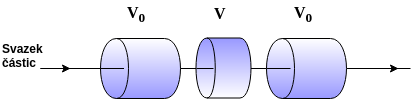
\includegraphics[width=.8\linewidth]{Figure/05/einzel.png}
\caption{Soustava třech elektrod s různým napětí.}
\label{einzel}
\end{figure}

Na Obr. \ref{pole} jsou schematický znázorněny siločáry elektrického pole vznikajícího v soustavě elektrod a chování svazku v tomto poli. Na prostřední elektrodu se v případě svazku elektronů dodává záporné napětí a vytváří se rozdíl potenciálů s každou s uzemněných okrajových elektrod. Po průchodu polem v rozmezí první a druhé elektrody svazek je zpomalen a rozptýlen v radiálním směru, dále po průletu druhou elektrodou svazek začíná být urychlován a stlačen radiálně, což vede k fokusaci do jednoho bodu, po proletění kterého, svazek znova defokusuje. Jelikož svazek je nejdřív zpomalen a potom urychlen, výsledná kinetická energie svazku po průchodu soustavou zůstává nezměněná. 
\begin{figure}[H]
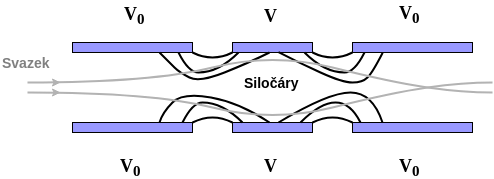
\includegraphics[width=.8\linewidth]{Figure/05/pole.png}
\caption{Schematické znázornění siločár elektrického pole v soustavě einzelových čoček.  }
\label{pole}
\end{figure}

Geometrie elektrod může být rozlišná a ovlivňuje fokusační vlastnosti soustavy, dalším důležitým parametrem působícím na chování svazku je napětí na elektrodách, v případě, že k dispozici je pouze soustava elektrod s určitou geometrii, polohu ohniska se dá zcela určit pomoci změny napětí na elektrodách. Při správném nastavení parametrů elektrostatické čočky nejenom fokusují svazek, ale také můžou ho urychlit, což jsme využili pro urychlování elektronového svazku v našem experimentu. 

Volbu geometrie a napětí na elektrodách jsme určili pomoci simulace soustavy v programu SIMION. 

